%!TEX root = ./template-skripsi.tex

\subsection{\textit{Sprint 10}}

	\textit{Sprint-10} dilakukan sepekan pada tanggal 25 oktober 2022 sampai dengan 1 november 2022. \textit{Story} kesepuluh pada \textit{product backlog} yaitu membuat fitur perpindahan antar kolam dipecah menjadi beberapa \textit{task} sebagai berikut.


 \begin{longtable}[c]{@{} |p{1cm}|p{4cm}|p{5cm}|p{3cm}| @{}}
 \caption{\textit{Sprint 10} \label{sprint10_table}}\\


 \hline
  \multirow{1}{=}{\centering{\textbf{No}}} & \multirow{1}{=}{\centering{\textbf{\textit{Story}}}} & \multirow{1}{=}{\centering{\textbf{\textit{Task}}}} & \multirow{1}{=}{\centering{\textbf{\textit{Status}}}}\\
 \endfirsthead

 \hline
  \multirow{1}{=}{\centering{\textbf{No}}} & \multirow{1}{=}{\centering{\textbf{\textit{Story}}}} & \multirow{1}{=}{\centering{\textbf{\textit{Task}}}} & \multirow{1}{=}{\centering{\textbf{\textit{Status}}}}\\
 \endhead

 \hline
 \endfoot

 \hline
 \endlastfoot

 \hline
 1 & Membuat fitur sortir kolam &  Membuat \textit{Mock-up UI} halaman list sortir, detail sortir, entry sortir &  selesai \\
 \hline
 2 & & Menerapkan \textit{Mock-up UI} halaman list sortir, detail sortir, entry sortir  ke Flutter & selesai\\
 \hline
 3 & & Mengintegrasikan halaman list soritr, entry soritr, detail soritr ke \textit{webservice} & selesai\\
 \hline
 \end{longtable}

Pada sprint kesepuluh ini story yang di pilih untuk di uraikan pada sprint kali ini adalah membuat fitur sortir. Tujuan dari \textit{sprint-10} ini adalah membuat fitur sortir ikan dan mengintegrasikan halaman tersebut dengan webservice yang sudah dibuat oleh penelitian Andri Rahmanto.

\begin{enumerate}[listparindent=2em]
	
	\item{\textit{Membuat Mock-up UI Fitur Sortir Kolam}}
	
	Pembuatan konten dan fitur yang terdapat pada \textit{mock-up UI} fitur sortir kolam dilakukan berdasarkan persetujuan product owner dan scrum master pada meeting sebelumnya. Mock-up UI dibuat menggunakan platform figma.
	
	\begin{figure}[H]
	\centering
	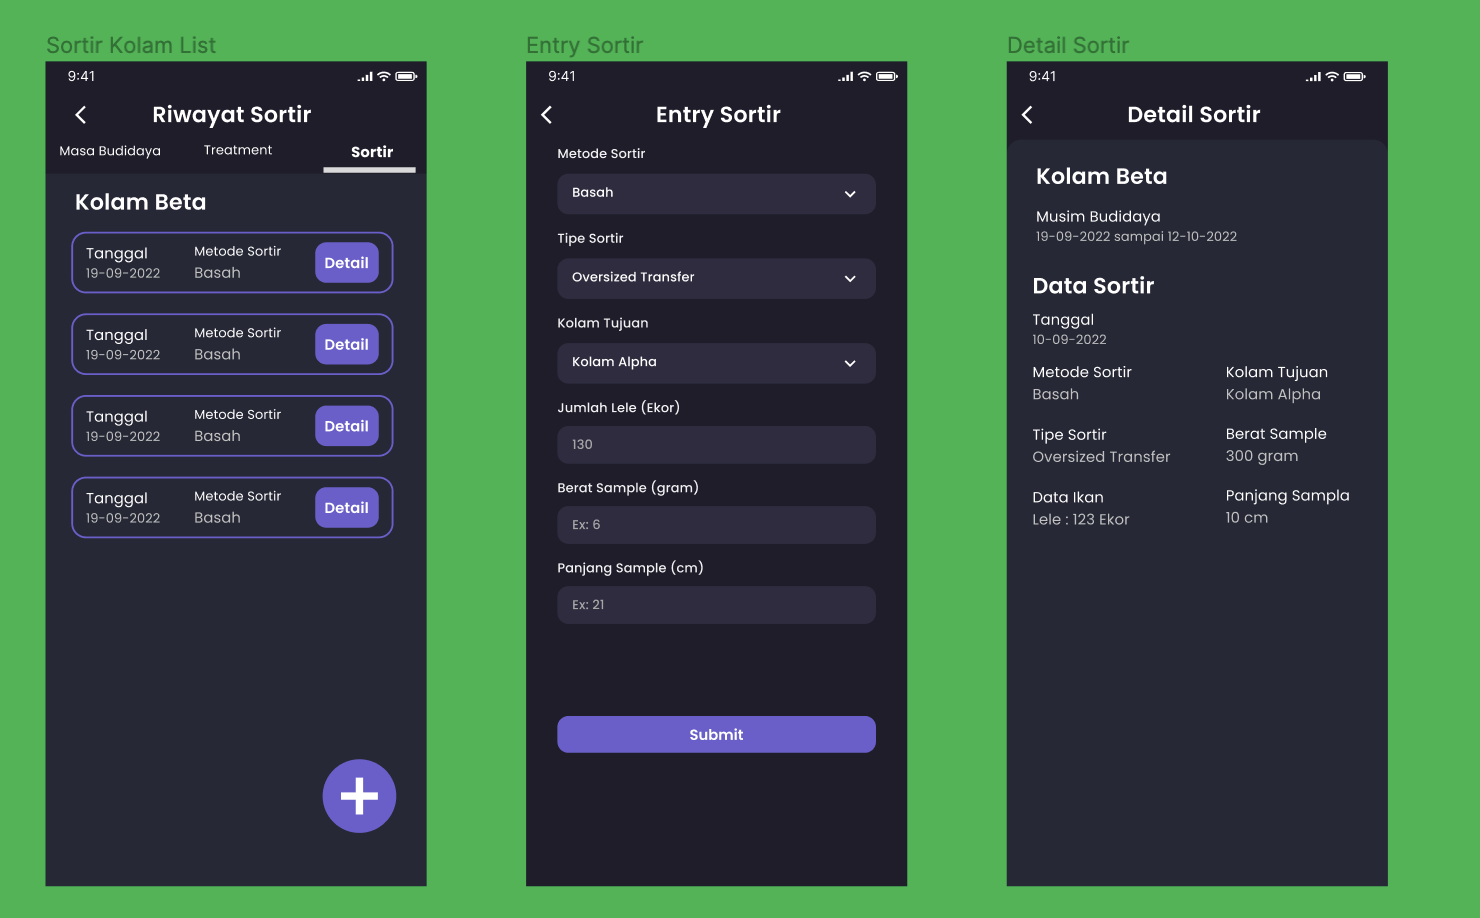
\includegraphics[keepaspectratio, width=10cm]{gambar/mockupsortir}
	\caption{\textit{Mock-up UI Fitur Sortir}}
	\label{gambar:mockupsortir}
	\end{figure}

	\item{\textit{Class Diagram}}
	
	Class Diagram menggambarkan kelas-kelas yang akan dipakai oleh sistem. Umumnya terdapat 3 kelas pada setiap module yaitu class model, controller, dan view. Pada sprint-10 penelitian kali ini penulis membuat 4 class yaitu model yang berwarna biru, view berwarna oranye, controller yang berwarna hijau, dan service yang berwarna kuning.
	 
	 \begin{figure}[H]
	 \centering
	 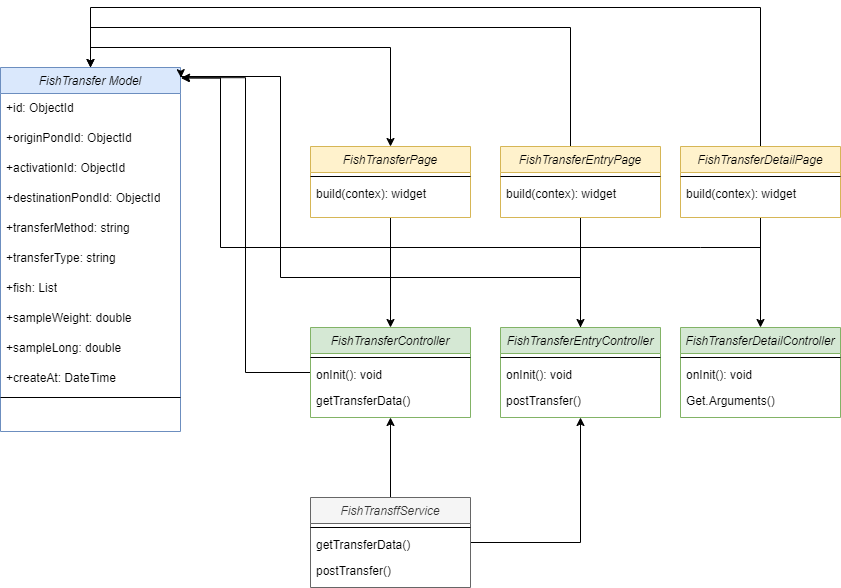
\includegraphics[keepaspectratio, width=6cm]{gambar/transfercd}
	 \caption{\textit{Class Diagram Fitur Sprint-10}}
	 \label{gambar:transfercd}
	 \end{figure}

	\item{\textit{Menerapkan Mockup-UI Fitur Sortir Kolam kedalam code flutter}}
	
	Setelah \textit{mock-up UI fitur Sortir kolam}, akan dilakukan pengimplementasian \textit{mock-up UI} ke dalam aplikasi menggukan flutter. Pada lampiran 11 terdapat source code dari implementasi fitur sortir yang dikelompokan berdasarkan halaman yang menghasilkan output halaman seperti dibawah ini.

	\begin{figure}[H]
		\centering
		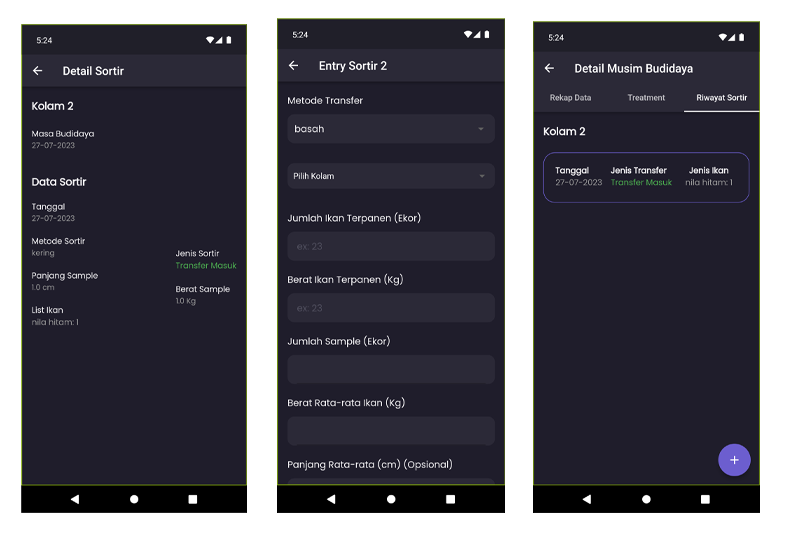
\includegraphics[keepaspectratio, width=8cm]{gambar/sssprint10}
		\caption{\textit{Output dari code pada sprint 10}}
		\label{gambar:sssprint10}
		\end{figure}

    \item{\textit{Mengitegrasikan fitur pencatatan kualitas air mingguan dengan webservice}}

	Sebelumnya, setiap data pada fitur masih berupa data dummy sehingga perlu diintegrasikan dengan webservice agar aplikasi dapat berjalan dengan data yang asli. Hal yang dilakukan dalam mengintegrasikan fitur sortir ikan dengan webservice terdapat pada lampiran 11.

  \item{Analisis \textit{User Experience}} 
 
  Pada halaman entry sortir kolam/transfer ikan, pembudidaya harus memasukan data yang diperlukan untuk melakukan sortir kolam/transfer ikan sesuai dengan kesepakatan saat meeting. Selain itu terdapat juga list mengenai data sortir kolam/transfer ikan yang telah dimasukan yang berisi informasi yang berhubungan dengan sortir kolam/transfer ikan. Terdapat pula halaman detail sortir kolam/transfer ikan yang berisi informasi yang lebih detail terkait sortir kolam/transfer ikan yang telah dilakukan.

\item{Sprint 10 Review dan Sprint 11 Planning}

Sprint 10 diakhiri dengan melakukan weekly meeting pada hari selasa dengan agenda melakukan review dan testing terkait hasil sprint 10 dan melakukan planning untuk sprint 11 dengan rincian:
\begin{enumerate}
	\item{\textit{Review dan Testing hasil dari sprint 10}}

	Telah dilakukan review dan testing oleh penulis selaku developer dengan Scrum Master. Setelah dilakukan testing, Scrum Master menyimpulkan bahwa fitur transfer/sortir ikam telah berjalan dengan baik.
	
  \begin{longtable}{| p{8cm} | c | c | l |}
    \caption{Unit testing Halaman Rekapitulasi Sortir.\label{table:unit_testing_rekapitulasi_sortir}}\\
    \hline
    \multirow{2}{*}{Skenario Pengujian} & \multicolumn{2}{l|}{Kesesuaian} & \multirow{2}{*}{Kesimpulan} \\ 
    \cline{2-3}
      & \multicolumn{1}{l|}{sesuai} & tidak sesuai & \\ 
    \hline
    \hline
    \endfirsthead
    \hline
    \multirow{2}{*}{Skenario Pengujian} & \multicolumn{2}{l|}{Kesesuaian} & \multirow{2}{*}{Kesimpulan} \\ 
    \cline{2-3}
      & \multicolumn{1}{l|}{sesuai} & tidak sesuai &  \\ 
    \hline
    \hline
    \endhead
    \hline
    \endfoot
    
    
    \hline\hline
    \endlastfoot
    Ketika menekan list data sortir, maka akan ditamplikan detail sortir & \Checkmark &  & Diterima \\ 
    \hline
    Saat ikon (+) ditekan maka akan menampilkan halaman entry sortir & \Checkmark &  & Diterima \\ 
    \hline
    ketika mengisi form sortir dengan data yang sesuai dan menekan submit, data sortir akan ditambahkan & \Checkmark &  & Diterima \\ 
    \hline
    \end{longtable}

	\item{\textit{Sprint Planning untuk Sprint 11}}
	
	Planning untuk sprint 11 yakni membuat fitur multi user pada aplikasi \textit{Assistive Aquaculture Breeding Management}.
\end{enumerate}
\end{enumerate}